\chapter{Métodos Iterativos para Zeros de Função}

Em muitas aplicações, as soluções buscadas se resumem a encontrar os zeros (ou raízes) de uma função. Entretanto, nem sempre é possível fazê-lo analiticamente, devido à natureza das componentes envolvidas na função como, por exemplo, funções polinomiais a partir do 3º grau, somas de funções trigonométricas e logarítmicas, entre outras. Nesse ínterim, recorremos então a maneiras de obter valores aproximados para tais raízes. 

Uma classe de métodos utilizados para aproximar raízes de funções são os \textbf{métodos iterativos}. A essência desses métodos está em, partindo de um chute inicial e de uma função apropriada $\varphi$, obter uma sequência $x_k$ onde cada termo é obtido do anterior recursivamente como $x_{k+1} = \varphi(x_k)$. Essa sequência, sob certas hipóteses, converge para a raiz $\xi$ da função.


Ao longo do capítulo, reservaremos o símbolo $\xi$ para representar raízes de funções.

\section{Localização de Raízes}

%Mais adiante no capítulo
Nos métodos que trataremos nesse capítulo, para garantir a convergência da sequência iterativa, é necessário que o primeiro termo esteja suficientemente próximo da raiz e, desse modo, faz-se necessário restringir as funções a intervalos que contenham raízes. Quando as funções envolvidas são contínuas, o resultado a seguir garante a existência de raízes em um intervalo [a,b] desde que as imagens dos extremos tenham sinais opostos.

\begin{prop}\label{c_tvi}%[Corolário do Teorema do Valor Intermediário]
Seja $f(x)$ uma função contínua no intervalo $[a, b]$. Se $f(a)f(b) < 0$, então há pelo menos uma raiz $\xi \in (a,b)$. Se, além disso, existir $f'(x)$ e $f'(x)$ preservar o sinal em $(a,b)$, então a raiz é única.
\end{prop} %para todo d entre f(a) e f(b) existe ao menos um f(c) = d %então para f(a) > 0 e f(b) < 0, existe pelo menos um f(c) = 0
Por exemplo, considere a função $f(x) = x^3 - 9x + 3$. Utilizando a Proposição \ref{c_tvi}, observamos que
\begin{itemize}
    \item $f(0)f(1) = -15 < 0$, portanto há raiz no intervalo (0, 1);
    \item $f(2)f(3) = -21 < 0$, portanto há raiz no intervalo (2, 3).
\end{itemize}
Além disso, a derivada de $f(x)$ é $f'(x) = 3x^2 - 9$, cujas raízes são $\pm \sqrt{3}$, então nos intervalos (-$\infty$, -$\sqrt{3}$), (-$\sqrt{3}$, $\sqrt{3}$) e ($\sqrt{3}$, $\infty$) o sinal da derivada é preservado. Portanto, nos intervalos $(a,b)$ e $(c,d)$ há apenas uma raiz.

\begin{figure}[h]
    \centering
    \includegraphics[height = 0.5\textwidth]{Imagens/corolário.png}
    \caption{Raiz entre A e B, e entre C e D}
    \label{fig:coro}
\end{figure}

\newpage

Outra forma de localizar raízes de uma dada função $f(x)$ é escrevê-la como a diferença entre as funções $g(x)-h(x)$, pois se $f(\xi) = 0$ temos que $g(\xi) - h(\xi) = 0$ ou, equivalentemente, $g(\xi) = h(\xi)$. Graficamente, $\xi$ é a abscissa do ponto de interseção entre as funções g(x) e h(x).

Da mesma função, podemos obter, por exemplo, as interseções entre $x$ e $x^3 - 8x + 3$
\begin{figure}[h]
    \centering
    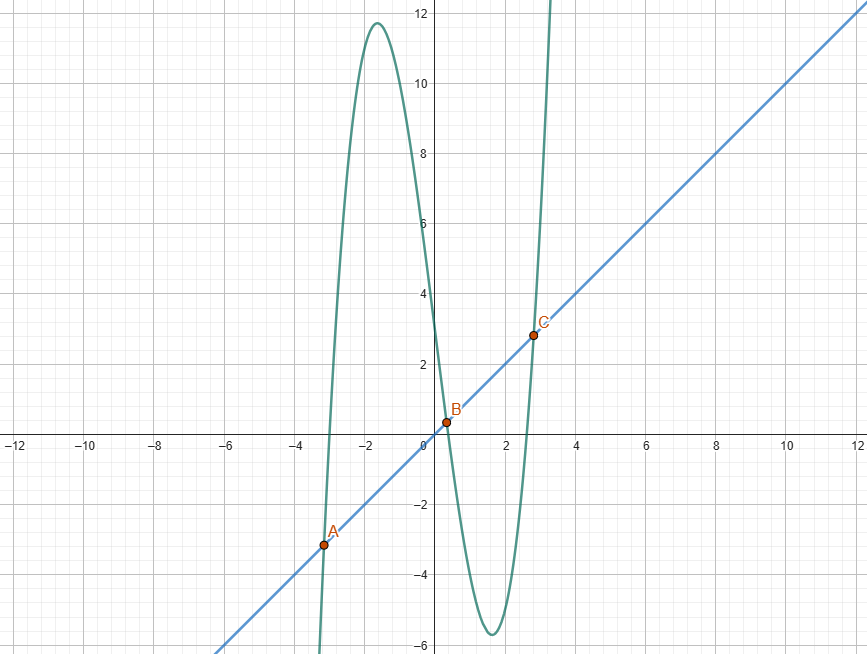
\includegraphics[height = 0.5\textwidth]{Imagens/interseções.png}
    \caption{Interseções entre x e $x^3 - 8x + 3$}
    \label{fig:inters}
\end{figure}

\section{Critério de Parada}
O processo é repetido até que a diferença entre duas iterações consecutivas seja inferior a uma tolerância pré-estabelecida ou até que um número máximo de iterações seja atingido.

\begin{itemize}
    \item $e_k = x_k - \xi$
    \item $e_k =  f(x_k) - 0$
\end{itemize}

\textcolor{blue}{Definir raiz aproximada}

\section{Método do Ponto Fixo}

O método do ponto fixo \emph{é um método iterativo} que %parte da ideia de que as interseções de duas curvas construídas a partir de uma função f(x) revelam suas raízes para então construir uma função $\varphi(x)$ e buscar suas interseções com a reta identidade, que 
transforma o problema de buscar as raízes de uma função $f(x)$ no problema de encontrar os pontos fixos de uma outra função $\varphi(x)$, denominada de \textbf{função de iteração de ponto fixo}. 
A partir dessa função de iteração, uma sequência é construída recursivamente começando em um valor inicial $x_0$ que convergirá para a raiz $\xi$ de $f(x)$, desde que sejam observadas certas condições sob a função $\varphi(x)$ e o dado inicial $x_0$.

%Após localizar um intervalo que contenha uma raiz pelos métodos expostos,
O primeiro passo é gerar funções de iteração $\varphi$ para $f(x)$, o que pode ser feito isolando $x$ na equação $f(x) = 0$. Por exemplo, manipulando a função $x^3 -9x + 3$  da seguinte forma 
\begin{equation*}
    x^3 - 8x + 3 = x 
\end{equation*} 
obtemos a função de iteração $\varphi(x) = x^3 - 8x + 3$. Com a mesma lógica, outras possíveis funções de iteração para $f$ são

\begin{multicols}{2}
\begin{itemize} %itemize (era enumerate)
    \item[a)] $\varphi_1(x) = \frac{x^3}{9} + \frac{1}{3}$
    \item[b)] $\varphi_2(x) = \sqrt[3]{9x-3}$
    \item[c)] $\varphi_3(x) = \frac{9}{x} - \frac{3}{x^2}$
    \item[d)] $\varphi_4(x) = \sqrt{9 - \frac{3}{x}}$
    \item[e)] $\varphi_5(x) = -\sqrt{9 - \frac{3}{x}}$
    \item[f)] $\varphi_6(x) = x^3 - 8x + 3$
\end{itemize}
\end{multicols}
A forma geral da função de iteração é 
\begin{equation}
    \varphi(x) = x + A(x)f(x) \label{it}
\end{equation}
com $A(\xi) \ne 0$.
%É necessário verificar então se as funções de iteração geradas respeitam essa condição de $A(\xi) \neq 0$. 
Por exemplo, a $\varphi_1 = \frac{x^3}{9} + \frac{1}{3}$ na forma geral ficaria 
\begin{equation*}
    \varphi_1(x) = x + \frac{1}{9}f(x)
\end{equation*}
\begin{comment}
    \varphi_1(x) &= x + \frac{1}{9}(x^3 - 9x + 3) \\
    \varphi_1(x) &= x + \frac{x^3}{9} - x + \frac{1}{3} \\
    \varphi_1(x) &= \frac{x^3}{9} + \frac{1}{3}
\end{comment}
em que $A(x) = \frac{1}{9}$. Nesse caso, pode-se observar que A($\xi) \neq 0$.

O resultado a seguir relaciona a raiz de uma função com pontos fixos de uma função de iteração associada a essa função. 

\begin{prop}
Seja $\xi$ uma raiz de uma função $f(x)$ e seja $\varphi(x)$ uma função de iteração associada a $f(x)$. Então, $f(\xi) = 0$ se, e somente se, $\varphi(\xi) = \xi$.
\end{prop}

%Provando primeiramente que a raiz da função é ponto fixo da função de iteração, $f(\xi) = 0 \Rightarrow \varphi(\xi) = \xi$. Começa-se calculando a função de iteração para a raiz $\xi$, isto é, $\varphi(\xi)$, obtendo então, pela forma geral, a raiz somada ao produto da função A pela função original $ \xi + A(\xi)f(\xi)$. Dado que $\xi$ é raiz de f(x), o valor da função calculado em $\xi$ é 0, portanto se tem $\xi + A(\xi) \cdot 0$; o que anula o produto com a função A, $\xi + 0$. Com isso, concluí-se que a função de iteração calculada na raíz é de fato igual a $\xi$.

\begin{proof}
($\Rightarrow$) Pela forma geral da função de iteração temos que $\varphi(\xi) = \xi + A(\xi)f(\xi)$. Uma vez que $f(\xi) = 0$, então $\varphi(\xi) = \xi$.

($\Leftarrow$) Começando novamente pela forma geral da função de iteração, temos que $\varphi(\xi) = \xi + A(\xi)f(\xi)$. Como $\varphi(\xi) = \xi$, concluímos que $A(\xi) f(\xi) = 0$. Tendo como hipótese que $A(\xi) \neq 0$, então $f(\xi) = 0$.
%ou seja, o ponto fixo $\xi$ da função de iteração $\varphi$ é raíz da função original $f(x)$. %q.e.d. (\textit{quod erat demonstrandum}, qual estava-se a demonstrar).
\end{proof}

%\newpage
\textcolor{blue}{Aqui, antes de ir para o resultado principal, dar exemplos de funções de iteração que fazem a sequencia convergir e divergir. Inserir gráficos assim como no livro da Vera.} \textcolor{green}{ok!}\\

Sob condições a respeito da função de iteração, sua derivada e o dado inicial, a convergência da sequência iterativa é garantida, como pode-se observar a seguir.
%Enfim é importante verificar se a função de iteração de ponto fixo respeita as condições para convergência.

\begin{teo}
    Seja $\xi$ uma raiz de f(x), isolada num intervalo I centrado nessa raiz. Considere uma função de iteração $\varphi(x)$ associada a f(x). Sob as seguintes hipóteses:
    \begin{itemize}\label{teoMPF}
        \item[i)] $\varphi(x)$ e $\varphi'(x)$ são contínuas em I,
        \item [ii)] $|\varphi'(x)| \leq M < 1$ em I,
        \item [iii)] $x_0 \in I$,
    \end{itemize}
    a sequência $x_{k+1} = \varphi(x_k)$ converge para a raiz $\xi$. 
\end{teo}
%Dada uma função $\varphi(x)$ ela é chamada de função de iteração, pois $\varphi(x_k) = x_{k+1}$ e através dessas iterações podemos buscar o ponto fixo dela na qual $x_k = \xi$. Provaremos a seguir que dada uma raíz $\xi$ de f(x) isolada num intervalo I centrado na mesma, a sequência recursiva $\varphi(x_k) = x_{k+1}$ converge para $\xi$ tendo: a função contínua e derivável, e sua derivada também contínua, no intervalo (a,b); o módulo (M) de sua derivada limitado e inferior a unidade no intervalo ($|\varphi'(x)| \leq M < 1$ $\forall x \in (a, b)$); e o primeiro valor da iteração no intervalo ($x_0 \in I$).
\begin{proof}
Como $x_{k+1} = \varphi(x_k)$, subtraindo $\xi$ de ambos os lados da igualdade e usando o fato de que $\varphi(\xi)=\xi$ temos
    \begin{equation}\label{difIt}
        x_{k+1} - \xi = \varphi(x_k) - \varphi(\xi).
    \end{equation}
    Pelo Teorema do Valor Médio (TVM) podemos escrever \\
    \begin{equation}\label{tvm}
        \varphi(x_k) - \varphi(\xi) = \varphi'(c_k) (x_k - \xi)
    \end{equation}
    com $c_k$ entre $x_k$ e $\xi$. Então, substituindo (\ref{tvm}) em (\ref{difIt}), temos
    \begin{align}\label{des}
        %x_{k+1} - \xi &= (x_k - \xi) \ \varphi'(c_k) \\
        |x_{k+1} - \xi| &= |(x_k - \xi) \ \varphi'(c_k)| \nonumber \\
        &= |x_k - \xi| \ |\varphi'(c_k)| \\
        &< |x_k - \xi| \nonumber
    \end{align}
    uma vez que $|\varphi'(x)| < 1$. Como $x_0 \in I$, podemos concluir que $x_k \in I$ para todo $k$ já que, por (\ref{des}), $|x_k - \xi| < |x_0 - \xi|$. 

    Na sequência, provaremos que $x_k$ converge para a raiz $\xi$. Vamos começar mostrando que 
    \begin{equation}\label{lab2}
        |x_1 - \xi| \leq M \ |x_0 - \xi|.
    \end{equation}
    Observe que, como $x_1=\varphi(x_0)$, temos que $x_1 - \xi = \varphi(x_0) - \varphi(\xi)$. Pelo Teorema do Valor Médio temos que $\varphi(x_0) - \varphi(\xi) = (x_0 - \xi) \ \varphi'(c_0)$, para algum $c_0$ entre $x_0$ e $\xi$. Uma vez que $|\varphi'(x)| \leq M$ no intervalo $I$, a seguinte desigualdade é válida
    \begin{align*}
        |x_1 - \xi|&= |x_0 - \xi| \ |\varphi'(c_0)|\\
        &\leq M \ |x_0 - \xi|
    \end{align*}
    e provamos a desigualdade (\ref{lab2}).
    %\begin{align*}
    %    |x_1 - \xi| &= |\varphi(x_0) - \xi| \\
    %    \text{Pelo TVM,} \ \varphi(x_0) - \xi &= (x_0 - \xi) \ \varphi'(c_0) \text{, com $c_0 \in (x_0, \xi)$} \\
    %    |x_1 - \xi| &= |x_0 - \xi| \ |\varphi'(c_0)| \\
    %    \text{Como $|\varphi'(x)| \leq M$,} \ |\varphi'(c_0)| \ |x_0 - \xi| &\leq M \ |x_0 - \xi| \\
    %    |x_1 - \xi| &\leq M \ |x_0 - \xi|
    %\end{align*}
    De modo similar prova-se que $|x_2 - \xi| \leq M \ |x_1 - \xi|$ que, combinado com (\ref{lab2}), implica que $|x_2 - \xi| \leq M^2 \ |x_0 - \xi|$. Repetindo o processo k vezes pode-se concluir que
    \begin{equation}\label{lim0}
        |x_k - \xi| \leq M^k \ |x_0 - \xi|.
    \end{equation}
    Como $0 < M < 1$, se k tende a infinito, $M^k$ tende a 0 e, portanto, $M^k \ |x_0 - \xi|$ também tende a 0. Assim, provamos que
    %\begin{align*}
    %\lim_{k \to \infty} |x_k - \xi| &\leq M^k \ |x_0 - \xi| \\
    %\lim_{k \to \infty} |x_k - \xi| &\leq 0 \ |x_0 - \xi| \\
    %\lim_{k \to \infty} |x_k - \xi| &= 0 \ \text{logo, }
    %\end{align*}
    \begin{equation}
        \lim_{k \to \infty} x_k = \xi, \label{conv.mpf}
    \end{equation}
    ou seja, $x_k$ converge para a raiz.
\end{proof}


% $\varphi'(x) = \frac{x^2}{3}$ \\ $|\varphi'(x)| < 1$ para $x \in (-\sqrt{3}, \sqrt{3})$ 

\subsection{Ordem de convergência}

\textcolor{blue}{Dizer aqui o que significa na prática a ordem de convergência de um método. Perceba que pela definição ele está ligado ao erro cometido no processo iterativo.}
\begin{df}
    Seja $\{x_k\}$ uma sequência que converge para $\xi$ e $e_k = x_k - \xi$ o erro na k-ésima iteração.
    %um num. p e uma cte. C
    Se existirem $p > 1$ e $C > 0$ tais que $\lim_{k \to \infty} \frac{|e_{k+1}|}{|e_k|^p} = C$, então $p$ é chamada de \emph{ordem de convergência} da sequência e $C$ é a \emph{constante assintótica de erro}.
\end{df}

\begin{comment} sobre p
A ordem de convergência $p$ de um método iterativo fornece uma informação sobre a rapidez de convergência do processo, pois podemos reescrever (\ref{conv}) como $|e_{k+1}| = C |e_k|^p$ para k tendendo ao infinito. 

Uma vez que a sequência {$x_k$} é convergente, $e_k$ tende a 0 quando $k$ tende ao infinito, portanto, quanto maior for $p$ mais próximo de 0 estará $C|e_k|^p$ (independente de C), implicando numa convergência mais rápida da sequência. Assim, se dois processos iterativos resultam em sequências {$x_k^1$} e {$x_k^2$}, ambas convergindo para $\xi$, com suas respectivas ordens de convergência $p_1$ e $p_2$, se $p_1 > p_2 \geq 1$, o processo que gera a sequência {$x_k^1$} converge mais rapidamente.
\end{comment}

$|e_{k+1}| \approx C |e_k|^p$

\begin{prop}
    Se 
    \begin{equation}\label{conv}
        \lim_{k \to \infty} \frac{e_{k+1}}{e_k} = C, \ 0 \leq |C| < 1,
    \end{equation}
    então a convergência é pelo menos linear. O MPF tem convergência pelo menos linear.
\end{prop}
\begin{proof}
Partindo de (\ref{difIt}) e (\ref{tvm}), e tomando o  limite com k tendendo a infinito, podemos escrever (\ref{conv}) como
\begin{comment}
\begin{align*} só pra lembrar o que são as refs
    x_{k+1} - \xi &= \varphi(x_k) - \varphi(\xi) \\
    %\varphi(x_k) - \varphi(\xi) &= \varphi'(c_k) (x_k - \xi) \\
    %x_{k+1} - \xi &= \varphi'(c_k) (x_k - \xi) \\
    &= \varphi'(c_k) (x_k - \xi)
\end{align*}
\end{comment}
\begin{equation*} %\frac{x_{k+1} - \xi}{x_k - \xi} = \varphi'(c_k)
    \lim_{k \to \infty} \frac{x_{k+1} - \xi}{x_k - \xi} = \lim_{k \to \infty}\varphi'(c_k)
\end{equation*} %se $x_k$ converge para $\xi$ então $c_k$ também converge para $\xi$.
com $c_k$ entre $x_k$ e $\xi$
%, obtendo $C = \varphi'(\xi)$, pois, assim como $x_k$, $c_k$ converge para $\xi$
. %análogo ao uso de (2.4) antes de (2.5), certo?
\begin{comment}
\begin{align*} sem ser inline
    \lim_{k \to \infty} \frac{x_{k+1} - \xi}{x_k - \xi} &= \lim_{k \to \infty}\varphi'(c_k) \\
    &= \varphi'(\lim_{k \to \infty} c_k) \\
    &= \varphi'(\xi),
\end{align*}
ou seja,
\begin{equation*}
    \lim_{k \to \infty} \frac{e_{k+1}}{e_k} = \varphi'(\xi)
\end{equation*}
\end{comment} 
%é necessário, mostrar que \varphi'(\lim_{k \to \infty} c_k) = \varphi'(\xi)? uma vez que o que importa é que \varphi'(x) < 1 independente do x
Como por hipótese $\varphi'(x) < 1$ então $|C| < 1$, portanto, a convergência do MPF é pelo menos linear.
\end{proof}
    
%--------------------------------------------------------------------
\section{Método de Newton-Raphson}

O método de Newton é um caso particular do \textbf{Método do Ponto Fixo}, amplamente utilizado para encontrar raízes reais de funções não lineares, cuja ordem de convergência é pelo menos quadrática. A função de iteração específica para este método produz uma sequência em que cada termo $x_{k+1}$ corresponde geometricamente à interseção da reta tangente a $f(x)$ no ponto $(x_k, f(x_k))$ com o eixo x. 

No método do ponto fixo, vimos que se a função satisfaz o Teorema \ref{teoMPF} a sequência $x_{k+1} = \varphi(x_k)$ converge para $\xi$. Além disso, a desigualdade (\ref{lim0}) na demonstração desse resultado nos diz que quanto menor for $|\varphi'(x)|$, mais rápido a sequência $\{x_k\}$ converge.

Dada uma função \(f(x)\), o processo parte de uma estimativa inicial \(x_0\) e aplica a seguinte fórmula iterativa, a partir da escolha da derivada em (\ref{it})
\begin{equation}
    x_{k+1} = x_k - \frac{f(x_k)}{f'(x_k)},
\end{equation}
onde \(f'(x_k)\) é a derivada da função \(f\) avaliada em \(x_k\).
Para que o método convirja para a raiz correta, é necessário que \(f(x)\) seja continuamente diferenciável em uma vizinhança da raiz e que \(f'(x) \neq 0\) nessa região. Além disso, a escolha adequada do ponto inicial \(x_0\) é crucial para garantir a convergência do método.

Aplicando a derivada na forma geral de $\varphi$ pela regra da cadeia obtemos $\varphi'(x) = 1 + A'(x)f(x) + A(x)f'(x)$, calculando ela na raiz resta $\varphi'(x) = 1 + A(\xi)f'(\xi)$. Por hipótese, a $\varphi'(\xi) = 0$, pelo que temos $A(x) = \frac{-1}{f'(x)}$. Portanto, a forma da função de iteração do método de Newton-Raphson é 
\begin{equation*}
    \varphi(x) = x - \frac{f(x)}{f'(x)}
\end{equation*}
\begin{comment}
\begin{align*}
    \varphi(x) &= x + A(x)f(x) \\
    \varphi'(x) &= 1 + A'(x)f(x) + A(x)f'(x) \\
    \varphi'(x) &= 1 + A(\xi)f'(\xi) \\
    0 &= 1 + A(\xi)f'(\xi) \\
    -1 &= A(\xi)f'(\xi) \\
    \frac{-1}{f'(\xi)} &= A(\xi) \\
    \frac{-1}{f'(x)} &= A(x) 
\end{align*}
\begin{align*}
    \varphi(x) &= x - \frac{f(x)}{f'(x)} \\
    \varphi'(x) &= 1 - \frac{f'(x)f'(x) - f(x)f''(x)}{[f'(x)]²} \\
     &= 1 - \frac{[f'(\xi)]² - f(\xi)f''(\xi)}{[f'(\xi)]²} \\
     &= 1 - \frac{[f'(\xi)]²}{[f'(\xi)]²} \\
     &= 0
\end{align*}
\end{comment}
desde que $f'(x) \neq 0$.

\subsection{Demonstração Geométrica}
\subsection{Convergência}
\begin{teo}
    Sejam $f(x)$, $f'(x)$ e $f''(x)$ contínuas num intervalo $I$ que contém a raiz $\xi$ de $f$, supondo $f'(\xi) \neq 0$. Então, existe um intervalo $\overline{I} \subset I$, contendo a raiz $\xi$, tal que $x_0 \in \overline{I}$, a sequência ${x_k}$ gerada pela função de iteração $\varphi(x) = x - \frac{f(x_k)}{f'(x_k)}$ convergirá para a raiz.
\end{teo}
\begin{proof}\label{teoNR}
    Sendo o método de Newton-Raphson um caso particular do MPF, basta provar que para $\varphi(x) = x - \frac{f(x)}{f'(x)}$ as hipóteses do Teorema \ref{teoMPF} são satisfeitas. 
    
    Primeiramente, observe que $\varphi'(x) = \frac{f(x)f''(x)}{[f'(x)]^2}$. Como $f'(\xi) \neq 0$ e $f'(x)$ é contínua em I, é possível obter $I_1 \subset I$ tal que $f'(x) \neq 0$ no intervalo $I_1$. Assim, a função $f$ e suas derivadas primeira e segunda são contínuas em $I_1$ e, consequentemente, a função de iteração e sua derivada também.
    
     Uma vez que a $\varphi'(x)$ é contínua em $I_1$ e $\varphi'(\xi) = 0$, é possível escolher $I_2 \subset I_1$ de modo que $|\varphi'(x)| < 1$ em $I_2$ tendo $\xi$ como centro do novo intervalo.

    Por fim, tomando, $\overline{I} = I_2$, satisfazem-se as hipóteses do Teorema \ref{teoMPF}.
\end{proof}
\subsection{Ordem de Convergência}
No MPF espera-se uma ordem de convergência ao menos linear, entretanto ao escolher uma função de iteração que satisfaça $\varphi'(\xi) = 0$, provaremos que sua ordem de convergência será ao menos quadrática.
\begin{prop}
    A ordem de convergência do método de Newton é pelo menos quadrática.
\end{prop}
\begin{proof}
    Suporemos todas as hipóteses do Teorema \ref{teoNR}. %(de Convergência do Método de Newton-Raphson), temos
    Partindo de $x_{k+1} = x_k - \frac{f(x_k)}{f'(x_k)}$, subtraindo $\xi$ em ambos os lados da igualdade, obtemos
\begin{equation} \label{eMNR}
    e_{k+1} = e_k - \frac{f(x_k)}{f'(x_k)} 
\end{equation}
O polinômio de Taylor de grau 2 para $f(x)$ centrado em $x_k$ é
\begin{equation*}
    f(x) = f(x_k) + f'(x_k)(x - x_k) + \frac{f''(c_k)}{2}(x-x_k)^2
\end{equation*}
com $c_k$ entre $x$ e $x_k$.
%$-(x-x_k)$
Assim, $f(\xi) = f(x_k) - f'(x_k)(x_k - \xi) + \frac{f''(c_k)}{2}(x_k-\xi)^2$,
tomando $x = \xi$, dado que $f(\xi) = 0$, dividindo a equação pela derivada de $f$ temos
\begin{align*}
    \frac{f''(c_k)}{2f'(x_k)}e_k^2 &= e_k - \frac{f(x_k)}{f'(x_k)} \\
    \frac{f''(c_k)}{2f'(x_k)}e_k^2 &= e_{k+1} \\
    \frac{e_{k+1}}{e_k^2} &= \frac{1}{2} \frac{f''(c_k)}{f'(x_k)}
\end{align*}
\begin{align*}
    \lim_{k \to \infty} \frac{e_{k+1}}{e_k^2} &= \lim_{k \to \infty} \frac{1}{2} \frac{f''(c_k)}{f'(x_k)} \\
     &= \frac{1}{2} \frac{f''[\lim_{k \to \infty} (c_k)]}{f'[\lim_{k \to \infty} (x_k)]} \\
     &= \frac{1}{2} \frac{f''(\xi)}{f'(\xi)} \\
     &= \frac{1}{2} \varphi''(\xi) \\ %mostrar que é \varphi''
     &= C
\end{align*}
%\frac{f(x_k)}{f'(x_k)} &= e_k - \frac{f''(c_k)}{2f'(x_k)}e_k^2
\end{proof}
\subsection{Ciladas}
O Método de Newton é amplamente utilizado na prática devido à sua rapidez e precisão em condições ideais. Contudo, ele pode falhar ou convergir para raízes incorretas se essas condições não forem satisfeitas. 
\subsection{Fractais}